Hybrid testing method can help to reduce the memory overhead by limiting the number of states to an acceptable level. However, as mentioned in Section~\ref{sec:introduction}, symbolic pointers and loops will quickly generate lots of useless states that may not increase the coverage but take too much proportion of the states budget.

To address the large number of states forked from symbolic pointers, we proposed a novel \textit{lazily concretization} of symbolic pointers which can not only reduce the number of states but also guarantee the coverage. 
For symbolic loops, we introduced an optimization (i.e., \textit{symbolic loop bucket}) based on the loop bucket in AFL to control the forking in symbolic loops. By doing this, the execution can go through the symbolic loops and penetrate into deeper code areas.
Both of the two improvements will be discussed in the following sections in detail.

\begin{figure}
\centering
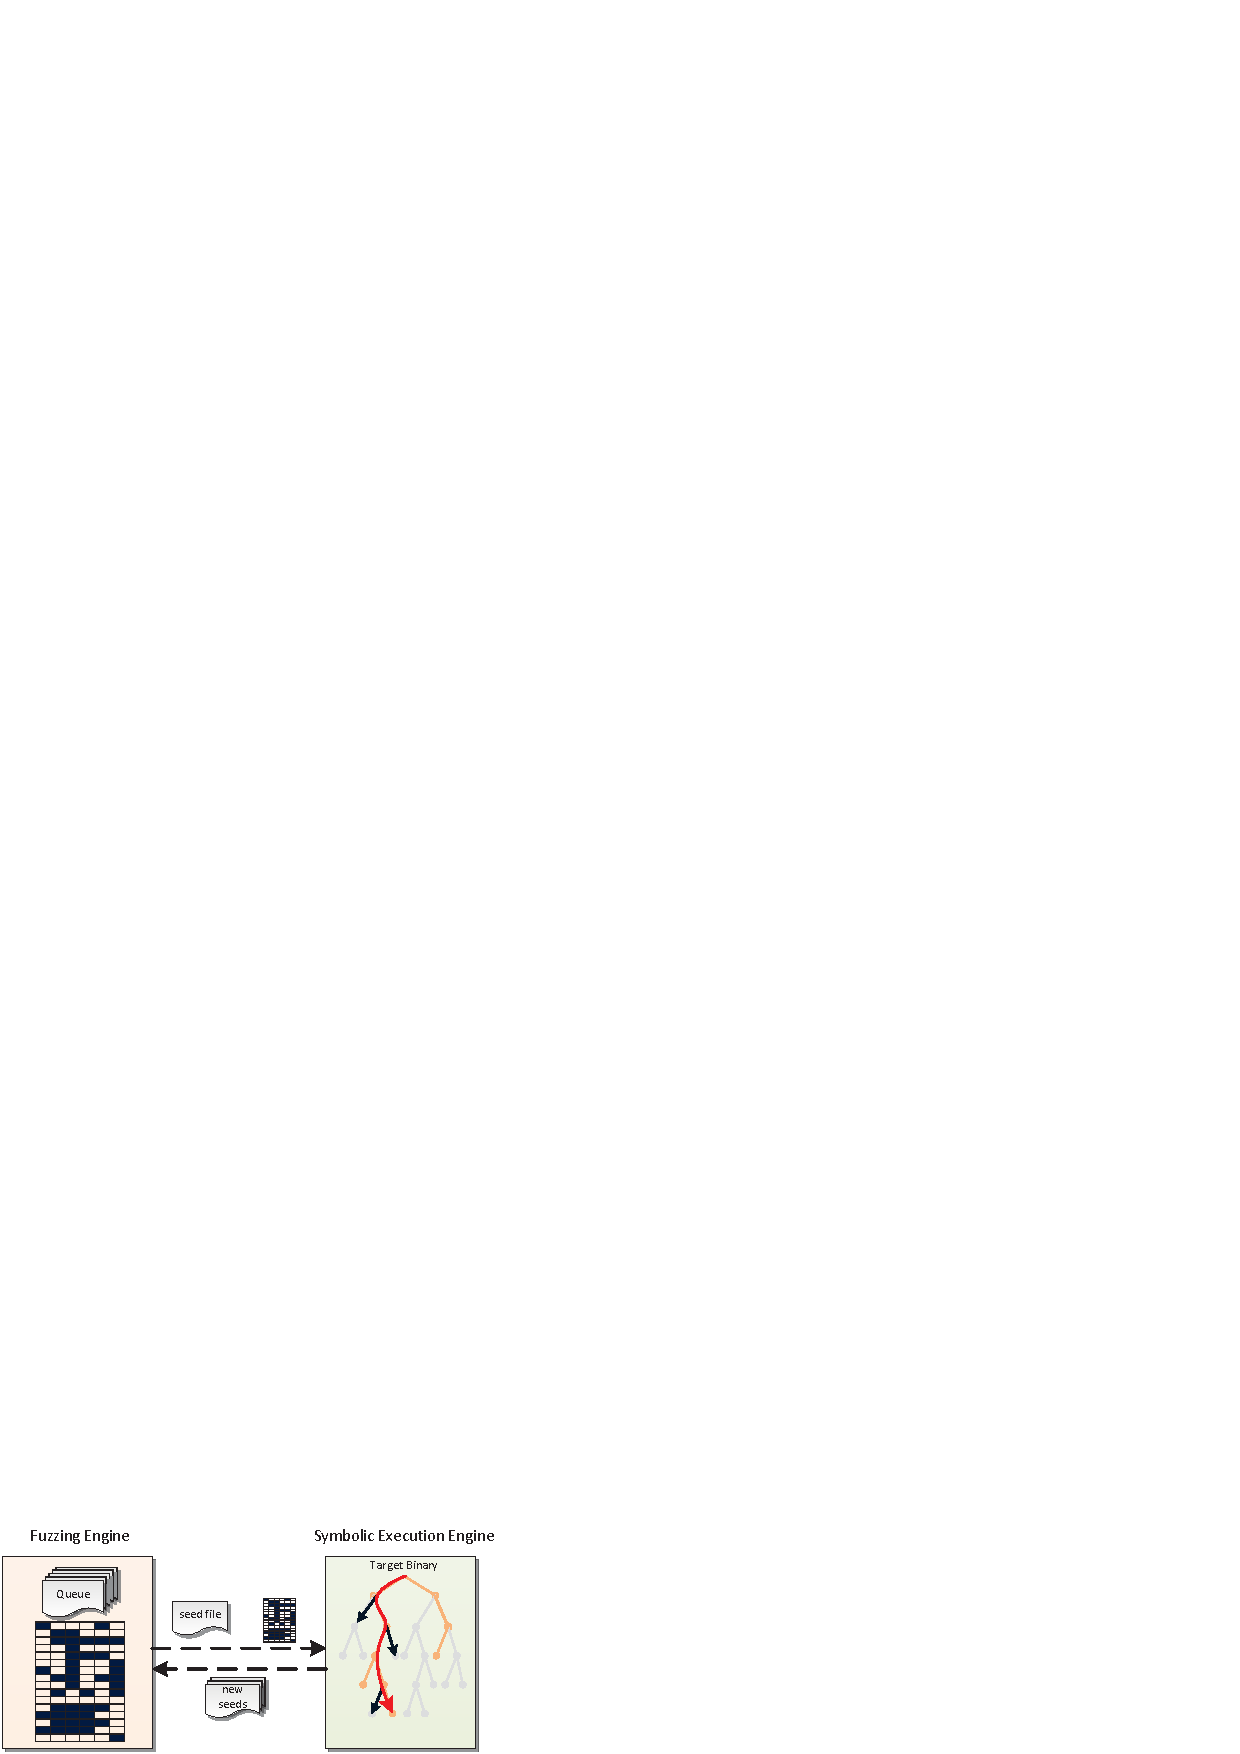
\includegraphics[width=0.7\textwidth]{figures/s2e-assist.pdf} 
\caption{Symbolic execution assisted fuzz testing.}\label{s2e-assist}
\end{figure}

\subsection{Lazy Concretization of Symbolic Pointer}
The code snippet in Listing~\ref{RE-LCSP} shows the basic symbolic pointer problem in symbolic execution. 
The first parameter (i.e., \texttt{buf}) of function \texttt{looks\_ascii} points to the memory that contains symbolic input data. The \texttt{nbytes} parameter is a concrete value that denotes the size of memory buffer pointed by \texttt{buf}. \texttt{ubuf} is the shadow buffer which is used for further process. 
Function \texttt{looks\_ascii} tries to determine whether each character of the symbolic input data appears in plain ASCII text at Line 18, and returns immediately once a non-plain ASCII text character appears. 
Since \texttt{buf[i]} has 256 possible values (\textit{unsigned char}) initially, so if the symbolic engine forks state for each possible value (i.e., full symbolic memory model), the total number of states forked from at Line 18 will quickly reach to $256^{nbytes}$ which raises ``path explosion'' problem. And the bug nested at Line 26 will be triggered only when the states that satisfy the path condition is scheduled. For example, suppose \texttt{nbytes} is 4, then worst case is that the bug can only be triggered after all of $256^4=4294967296$ states are scheduled.

When given a symbolic pointer, based on different memory models, different handle process can be taken. For example, in \textbf{full symbolic memory model}, each possible value of such pointer will fork a corresponding state \cite{song2008bitblaze, thakur2010directed, brumley2011bap, trtik2014symbolic}. There also exists a strategy namely \textit{address concretization} which will concretize the pointer to a single specific address \cite{godefroid2005dart, burnim2008heuristics}. Obviously, the full symbolic memory model will raise the serious state explosion (as mentioned before) and the address concretization may lose some interesting paths. To mitigate the scalability problems of full symbolic memory model and the loss of interesting paths of address concretization, a \textbf{partial symbolic memory model} has been proposed to make a trade-off \cite{cha2012unleashing, avgerinos2014exploiting, Shoshitaishvili_firmalice-automatic}. The partial symbolic memory model tries to concretize all symbolic pointer write operation and treats all symbolic pointer read operation as full symbolic memory model. However, because the instruction at Line 18 is the read operation, so partial symbolic memory model will still fork $256^{nbytes}$ states and raise the ``path explosion'' problem.

The \textit{lazy forking} strategy in S2E is proposed to avoid maintaining expensive symbolic pointers and large states number by forking a pending state in concolic execution \cite{chipounov2011s2e}. 
For example, for the instruction at Line 18 in Listing~\ref{RE-LCSP}, suppose the concrete value of \texttt{buf[i]} for $i\in[0,1,2,3]$ is \texttt{`A'}. 
Then the lazy forking will try to fork the current state to two states, one with a \textit{hard constraint} expressed as $\texttt{buf[i]}=\texttt{`A'}$ and the other one with a \textit{soft constraint} expressed as $\texttt{buf[i]}\neq\texttt{`A'}$.
By doing this, the ``path explosion'' problem is postponed to later moment. For example, new states will be only forked after the current state is terminated when using DFS search strategy.
\lstinputlisting[label={RE-LCSP}, language=C,style=c,caption={A motivating code that contains symbolic pointer dereference.}]{codes/real-eaxmple-LSP.c} 

However, the forking at Line 24\&25 will fail for the state with hard constraint. And the bug at Line 26 will be triggered only after enumerating all possible values for \texttt{buf[0]}, \texttt{buf[1]}, \texttt{buf[2]}, and \texttt{buf[3]}. So even though the lazy forking can ease the ``path explosion'' problem, it still needs to take longer time to trigger some interesting paths. This will bring performance loss as the objective of symbolic execution is to assist fuzz testing to uncover more paths as soon as possible in hybrid testing. 
To mitigate this problem, we introduce a novel method \emph{lazy concretization of symbolic pointer} (LCSP) which is built on top of lazy forking. The detailed algorithm of LCSP is shown in Algorithm~\ref{LCSP}.

\begin{algorithm}
  \caption{Lazy Concretizatin of Symbolic Pointer}
  \label{LCSP}
  \KwIn{Current State $S$, Pending States $S_P$ and Hard Constraint $C_H$}
  \KwOut{Testcase $t_{lsp}$ if success}
  $C_F = getFailedCondition()$\;
  $offs = S.getInputOffset(C_F)$\;
  \If{$S_P.find(offs) == S_P.end()$}
  {
    return $null$\;
  }
  $Conditions = S.getConditions().strip(C_H)$\;
  \ForEach{$s_p$ in $S_P.find(offs)$}
  {
    $s_{tmp} = s_p.clone()$\;
    $s_{tmp}.addConstraint(Conditions)$\;
    $s_{tmp}.addConstraint(C_F)$\;
    $(success, t_lsp) = s_{tmp}.generateTestcase()$\;
    \eIf{$success$}
    {
      return $t_{lsp}$;
    } {
      continue;
    }
  }
  return $null$\;
\end{algorithm}
  
When performing lazy forking, all the states whose path constraints contain the soft constraints will be collected into \emph{Pending States}. And the pending states are grouped by the input offsets that affect the corresponding soft constraint. 
Then when the symbolic execution engine fails to fork at the branch that depends on soft constraints, the failed condition will be inspected to extract the input offsets that affect this branch (Line 1\&2). LCSP ignores the case that the fork failure does not result from the lazy forking (Line 3$\sim$5). Then we extract all the related conditions in path constraint except for the hard constraint (Line 6), and then these conditions will be added to the pending states(Line 8\&9). Meanwhile, in order to generate the test case that satisfies the failed condition, the failed condition will be also added to the pending states (Line 10). After adding all related conditions, the symbolic execution engine will try to generate a new test case (Line 11), and once the generation successes, the test case $t_{lsp}$ will be sent to the fuzzer to find more paths.

For the motivating code in Listing~\ref{RE-LCSP}, suppose \texttt{nbytes} is 5. Then when symbolic execution reaches Line 24, there will be five states in the system, including one execution state $S_0$ and four pending states ($P_1$, $P_2$, $P_3$, $P_4$, and $P_5$). 
Then path constraint for each states is shown in Table~\ref{table:path-conditions}.

\begin{table}
  \caption{\label{table:path-conditions}Path Constraint for each state when reaching Line 24}
  \centering
	\begin{tabular}{p{2cm}<{\centering} p{1.5cm}<{\centering} p{1.5cm}<{\centering} p{1.5cm}<{\centering} p{1.5cm}<{\centering} p{1.5cm}<{\centering}}
		\toprule
		State  & buf[0] & buf[1] & buf[2] & buf[3] & buf[4]\\ 
		\midrule
		$S_0$  &  $=0x41$ & $=0x41$ & $=0x41$ & $=0x41$ & $=0x41$ \\
		$P_1$  &  $\neq0x41$ & null & null & null & null \\
		$P_2$  &  $=0x41$ & $\neq0x41$ & null & null & null\\
		$P_3$  &  $=0x41$ & $=0x41$ & $\neq0x41$ & null & null \\
		$P_4$  &  $=0x41$ & $=0x41$ & $=0x41$ & $\neq0x41$ & null \\
		$P_5$  &  $=0x41$ & $=0x41$ & $=0x41$ & $=0x41$ & $\neq0x41$ \\
		\bottomrule
	\end{tabular}
\end{table}

Obviously, $S_0$ will fail when trying to fork at Line 24\&25 ($C_{F}\leftarrow$ \{\texttt{buf[0]$=$`D' \& buf[1]$=$`E' \& buf[2]$=$`A' \& buf[3]$=$`D'}\}). Based on Listing~\ref{LCSP}, the path conditions of $S_0$ except for the hard conditions will be tried to add to each pending state to generate new test case. 
After stripping the hard conditions, the \textit{Conditions} at Line 6 in Listing~\ref{LCSP} will be $\texttt{buf[4]}=\texttt{`A'}$. Then this \textit{Conditions} will be added to each pending state. For example, the path constraint of $P_1$ after adding such conditions will be \{\texttt{buf[0]$\neq$`A' \& buf[4]$=$`A' \& buf[0]$=$`D' \& buf[1]$=$`E' \& buf[2]$=$`A' \& buf[3]$=$`D'}\}. After solving this path constraint, we can successfully generate a test case that satisfies the condition at Line 24\&25 and triggers the bug at Line 26. 
An interesting point in our example is that $P_2$, $P_3$, $P_4$, and $P_5$ cannot successfully trigger this bug. This does not mean that these states are useless, for example, if the condition at Line 24\&25 is \{\texttt{buf[0]$=$`A' \& buf[1]$=$`B' \& buf[2]$=$`C' \& buf[3]$=$`D'}\}, then $P_2$ can successfully generate a corresponding test case that triggers the bug.

Based on this algorithm, we can generate at least one fresh test case that satisfies the failed condition where the fork failure occurs because of lazy forking. But we still need to prove this test case will steer the program to execute the same path with the original state and then covers the branch that fails in the original state. A quick execution consistency proof is explained as follows:

Let $P_A$ be the execution path of a state $A$ which contains the following branches:


\begin{center}
$P_A = (B_0,T) \rightarrow (B_1,T) \rightarrow (B_2,F) \rightarrow (B_3,T)
\rightarrow (B_4,F) \rightarrow (B_5,F) \rightarrow (B_6,F) \rightarrow (B_u,T)$
\end{center}

\noindent where $B_n$ refers to the $n$-th branch. $T/F$ means state $A$ takes the \emph{True/False} branch and $B_u$ denotes the branch where the forking fails because of the extra hard constraint. Assume that hard constraint is $var=0xAB$ which is originated from the lazy forking from $B_1$, and the conditions at $B_3$ and $B_5$ are also affected by $var$.

Suppose state $B$ is the corresponding pending state forked from $B_1$, and then, according to the LCSP algorithm in Listing~\ref{LCSP}, when state $A$ raises a fork failure at branch $B_u$, all the related constraints except the hard constraint will be added to state $B$. After that, the path constraint of state $B$ will be:

\begin{center}
$PC_B = \displaystyle ^\neg CB_u \cap ^\neg CB_1 \cap \bigcap\limits_{i=0,i \neq 1}^{6} CB_i$
\end{center}
\noindent where the $CB_i$ denotes the path condition at branch $B_i$. We need to prove the following formula.

\begin{center}
$\mathbb{Z} = \{var\arrowvert PC_B(var) = True\} \neq \emptyset$
\end{center}

As there are only two branches before $B_u$ that depend on $var$, so the expression $PC_B$ can be simplified to:
\begin{center}
$PC_B = ^\neg CB_u \cap ^\neg CB_1 \cap CB_3 \cap CB_5$
\end{center}

There are two possible cases for $CB_3 \cap CB_5$:
\begin{center}
case1: $CB_3 \cap CB_5 = (var = 0xAB)$

case2: $CB_3 \cap CB_5 \neq (var = 0xAB)$
\end{center}

Under the first case, the path to $B_u$ is only feasible when $var$ equals to $0xAB$. So the edge $(B_u, F)$ will never be satisfied (i.e., \emph{dead code}) because $(var = 0xAB) \subseteq CB_u$. For the second case, there must be at least one feasible solution for $var$ that satisfies with the soft constraint $^\neg CB_1$, so $^\neg CB_1 \cap \bigcap_{i=0,i \neq 1}^{6} CB_i$ can be evaluated to $True$ for some specified values of $var$. This has proved that there must be at least one test case under $PC_B$ that can steer the program to the forking failure point $B_u$.

Similarly, for branch condition $B_u$, there are also two possible cases:
\begin{center}
case1: $\displaystyle ^\neg CB_1 \cap \bigcap\limits_{i=0,i\neq 1}^6 CB_i \subseteq CB_u$

case2: $\displaystyle ^\neg CB_1 \cap \bigcap\limits_{i=0,i\neq 1}^6 CB_i \nsubseteq CB_u$
\end{center}

The first case, which can also be expressed as $^\neg CB_u \cap ^\neg CB_1 \cap \bigcap_{i=0,i\neq 1}^6 CB_i = \emptyset$, is the case of \emph{dead code}. And the second case can be transformed into:
\begin{center}
$\displaystyle ^\neg CB_u \cap ^\neg CB_1 \cap \bigcap\limits_{i=0,i\neq 1}^6 CB_i \neq \emptyset \implies \mathbb{Z} = \{var\arrowvert PC_B(var) = True\} \neq \emptyset$
\end{center}

\noindent which means there must be at least one feasible value that satisfies the false branch of $B_u$. So above all, we can draw a conclusion that our \emph{LCSP} algorithm can keep the execution consistency when $(B_u, F)$ is not dead code.

\subsection{Optimization for Symbolic Loop}
Symbolic loop, whose loop control variable depends on symbolic data, will cause serious ``path explosion'' problem as its loop times will range from 0 to infinite theoretically. 
Even though the hybrid testing method can ease the ``path explosion'' problem, but the states forked from the symbolic loop will quickly force the number of states to increase to the budget. 

\lstinputlisting[label={RE-SLB}, language=C,style=c,caption={A motivating example to demonstrate path explosion raised by symbolic loops.}]{codes/example-SLB.c} 

The code snippet in Listing~\ref{RE-SLB} demonstrates this problem. Function \texttt{verify\_file} reads the \texttt{length} of the raw data from the file at Line 10. Then from Line 15 to 20, it investigates each bytes in the raw data to determine whether there exists the descriptor of the ending (i.e., \texttt{0xFF}) through a loop structure. Suppose we have a concrete test case from the seed queue of the fuzzer and the length domain is \texttt{0x000000AA}. 
When performing symbolic execution, the \texttt{length} variable will be symbolic which will then raise the ``path explosion'' problem at Line 15. Because the possible value of \texttt{length} will be in the range of [0, $2^{32}-1$], so there will be $2^{32}$ states forked from Line 15. And in the worse case, each forked state can continue forking states which will quickly reach the states limitation. 
Most of the forked states from Line 15 will not contribute to code coverage in this example but only bring performance overhead, So the symbolic loops have to be carefully handled to avoid getting stuck at the loop spot. 

AFL utilizes \emph{Loop Bucket} mechanism to avoid collecting too many test cases which only affect the loop times into the seed queue \cite{online:afl}. It groups the loop times into 8 different buckets, i.e., [1, 2, 3, 4-7, 8-15, 16-31, 32-127, 128+]. Only changes happened between different buckets will be regarded as new behaviors. Based on this idea, we proposed a \textit{Symbolic Loop Bucket} (SLB) to handle the symbolic loop when performing hybrid testing. The algorithm of SLB is described in Algorithm~\ref{SLB}.

Loops are extracted from the target program by static analysis. These loops will be configured to symbolic execution engine to help it recognize loops in runtime. All the symbolic loops can be distinguished from the others by checking whether the loop exit condition is affected by symbolic data or not (Line 1$\sim$3). For the edge belong to symbolic loop, the uncovered loop buckets for this loop will be obtained by analyzing the \textit{Bitmap} mentioned before (Line 5). 
State forking is disabled in already covered loop buckets, and the program will loop for one more time (Line 16\&17). Once an uncovered bucket is reached, the corresponding test case will be generated and then this uncovered bucket will be removed from the uncovered loop buckets to avoid generating multiple test cases (Line 7$\sim$12). After generating test cases for all the uncovered buckets, the loop will be prohibited from being executed for more times. This can make sure that all the loop buckets will be covered without coming across with the ``path explosion'' problem.

%TODO: Refine the algorithm to demonstrate what if the concrete value is less/greater than 128.
\begin{algorithm}
  \caption{Symbolic Loop Bucket}
  \label{SLB}
  \KwIn{Configured Loops $L$, Current Edge $CE$ and Bitmap $B_p$}
  \KwOut{Generated test cases $t_{slb}$}  
  \If{not $IsaLoopCycleEdge(L,CE)$ or not $IsaSymLoop(CE)$}
  {
    return;
  }
  $loopTimes$ = 1\;
  $UBs$ = $ParseUncoveredBuckets(B_p)$\;
  \While{TRUE}
  {
    \ForEach{$ub$ in $UBs$}
    {
      \If{$loopTimes$ within $ub$}
      {
        $t_{slb}.add(GenerateTestcase())$\;
        $UBs$.$remove(ub)$\;
      }
    }
    \eIf{$UBs$ is $null$}
    {
      return $t_{lsb}$\;
    }{
      $ExecuteOneCycle()$\;
      $loopTimes += 1$\;
    }
  }
\end{algorithm}  

For the symbolic loop in Listing~\ref{RE-SLB}. Suppose previous test cases have covered the buckets of [1], [2], [3], and [4-7]. Then \textit{UBs} at Line 5 in Algorithm~\ref{SLB} will consist of [8-15], [16-31], [32-127], and [128+]. $\textit{loopTimes}=[1, 2, \cdots, 7]$ will not fork any new states according to Line 15 to 18. Then once the \textit{loopTimes} reaches 8 which belongs to an uncovered bucket [8-15], the engine forks a new state,  generates the corresponding the test case, and removes bucket [8-15] from \textit{UBs}. The execution engines will not fork new states until \textit{loopTimes} reaches 16, 32 and 128. Once all the loop buckets are covered, the forking in this symbolic loop will be disabled. It will continue cycling until \textit{loopTimes} reaches the concrete value of \texttt{length} (i.e., \texttt{0x000000AA}) and then execute deeper code areas.
